\section{Laser}\label{sec:laser}

A técnica de reconstrução baseada em laser é conhecida desde o século passado, pois oferecem uma alta qualidade geométrica de dados, os resultados são em tempo real e requer pouco tempo de captura de dados. 

Existem alguns tipos de reconstruções empregando lasers, baseados em volume (ressonância, tomografia, por exemplo \ref{fig:laservolume} ou em superfície (estereoscopia, {\it time of flight}, luz estruturada) . Neste caso, abordaremos o projeto de escaneamento da escultura de Michelangelo, David, que utiliza escaners baseados em superfícies, mais especificamente, utilizando luz estruturada.

\begin{figure}[!h]
	\centering
	%   \includegraphics[width=1.0\linewidth]{figs/3d-curve-sketch/system-diagram.eps}
	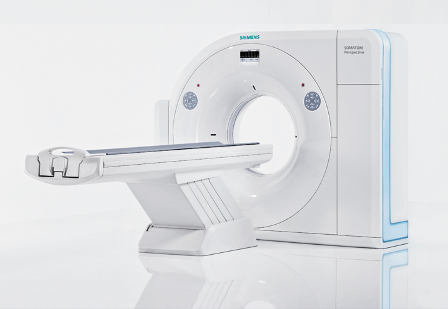
\includegraphics[width=1\linewidth]{figs/tomografia.png}
	\caption{%
	Exemplo de reconstrução à laser utilizando o método baseado em volume.
	%\cite{Cui:Theobalt:etal:PAMI2013,Pajdla:etal:ICCV2011}.
	}\label{fig:laservolume}
\end{figure}

Este projeto tem como motivação avançar a tecnologia de digitalização 3D e criar um acervo digital sobre alguns dos principais artefatos culturais. Foi utilizada uma tecnologia chamada de {\it rangefinder}, com uma equipe de mais de 30 professores, funcionários e estudantes da Universidade de Stanford desenvolveram algoritmos para combinar imagens de múltiplas gamas e cores, passaram os anos de 1998 e 1999 na Itália escaneando esclturas de Michelangelo. 

Pipeline:

O principal componente de {\it hardware} do sistema é um escaner de triangulação à laser, que é composto por 4 eixos motorizados, utiliza um laser, uma câmera de alcance, uma câmera de cores e uma luz branca, isso tudo acrescido de estruturas para estátuas grandes. O objetivo de um escaner deste porte era capturar marcas menores que um milímetro, das ferramentas utilizadas por Michelangelo em suas esculturas. 
Para isso foram testadas diversas resoluções, na qual foi decidido um espaçamento Y (ao longo da faixa do laser) de 1/4 mm e uma resolução Z (profundidade) de pelo menos duas vezes este valor. O que resultou em uma visualização de 14 cm de largura (ao longo da faixa do laser) por 14 cm de profundidade. Caso esta resolução fosse menor, as marcas de cinzelão ficariam borradas e se fosse maior, o conjunto de dados produzido seria gigantesco.
Felizmente, a maioria das estátuas feitas por Michelangelo foram esculpidas com um mármore encontrado em Carrara Statuario, uma pedra altamente uniforme, não direcional e constituída de grãos finos. Além disso, com exceção da "Noite", as esculturas não são polidas e cobertas por terra, o que aumenta a dispersão superficial e reduz a abaixo da superfície.
Neste contexto, a dispersão abaixo da superfície causa alguns problemas: não se pode assumir que a superfície é Lambertiana ideal (%CITAR LAMBERTIANO AQUI%
), mudou a forma com que a renderização dos modelos seriam feitos e diminuiu a qualidade de disposição de dados.
Calibração:
O objetivo de calibrar o aparato era encontrar um mapeamento de coordenadas 2D no seu alcance e cores para coordenadas 3D em um quadro de referência global. Idealmente, este quadro deve ser a estátua (estacionária). Porém não foi rastreado o aparato, ele tornou-se a própria referência. O mapeamento final foi realizado alinhando novas varreduras, com varreduras previamente existentes.
Para calibrar qualquer sistema, primeiramente escolhe-se um modelo matemático que se aproxime do comportamento do sistema, então estima-se parâmetros desse modelo medindo o comportamento do sistema. No caso do projeto de David, o modelo matemático natural era um modelo geométrico 3D parametrizado da cabeça digitalizada e do aparato. Se os componentes do sistema forem suficientemente independentes, a calibração pode ser dividida em estágios, correspondente a cada componente do sistema. Por isso o aparato foi construído pensando na rigidez (independência), pois particionar a calibração em etapas reduz o grau de liberdade em cada etapa, e com isso, o número de medidas necessárias para calibrar este estágio.
Em um sistema mecânico, também é reduzido o volume físico total na qual essas medidas de calibração devem ser tomadas. Além disso, uma calibração em etapas é menos suscetível a propagação de erros, pois caso uma calibração falhasse, seria apenas uma parte da calibração e não o sistema como um todo. No projeto de David, a calibração foi divida em seis etapas distintas:

\begin{enumerate}
\item{Um mapeamento 2D a partir de coordenadas de {\it pixels} das imagens da câmera para locais físicos na camada de laser}
\item{Transformação rígida 2D/3D do sistema de coordenadas da camada do laser para esferas de aço anexadas ao escaner da cabeça}
\item{Transformação rígida 3D para acomodar o rolamento do escaner da cabeça em 90° (ao remontá-lo) em relação ao conjunto de inclinação}
\item{A localização do eixo de rotação de inclinação e o mapeamento não-linear de movimento comandos para ângulos de rotação físicas}
\item{A localização do eixo de rotação panorâmico e o mapeamento de seus comandos de movimento para ângulos de rotação física}
\item{A localização do eixo de translação, que também depende de como o conjunto inclinação-panorâmico está montado no braço horizontal}
\end{enumerate}

O resultado da calibração pode ser descrito como uma concatenação de seis matrizes 4x4:

\left\[ translação horizontal \right\] \left\[ rotação panorâmica \right\] \left\[ rotação de inclinação \right\] \left\[ rotação de rolamento \right\] \left\[ laser para o escaner da cabeça \right\] \left\[ imagem para o laser \right\]

Calibração do sistema de cores:
Para corrigir a distorção geométrica na câmera de cores, foi fotografado um alvo de calibração planar que possui um certo número de {\it features} que, por sua vez, foram usados para calcular os parâmetros intrínsecos da câmera. Estão inclusos no modelo dois termos de distorção radial e dois termos de distorção tangencial que tem uma projeção de perspectiva fora do centro e uma escala possivelmente não uniforme (em X e Y) %CITAR[Heikkila..97].%

Para obter um mapeamento da câmera colorida para o escaner da cabeça, o alvo foi escaneado usando o laser e a câmera de alcance. Uma vez que o escaner retornou a intensidade refletida pelo laser, bem como a profundidade, pode-se calcular as coordenadas 3D de cada ponto da {\it feature}.

Para corrigir os efeitos radiométricos espaciais, incluindo o aspecto de vinheta das lentes, a não uniformidade angular, o declínio da lei quadrada inversa dos holofotes e a não uniformidade espacial na resposta do sensor, foi fotografado um cartão branco sob o holofote e construída uma tabela de correção de intensidade por pixel.
% Depois de testar várias resoluções, decidimos um espaçamento de amostra Y (ao longo da faixa laser) de 1/4 mm e uma resolução Z (profundidade) pelo menos duas vezes esta multa 1. Isso nos deu uma visão de 14 cm de largura (ao longo da faixa a laser ) por 14 cm de profundidade. Em retrospectiva, ficamos satisfeitos com a resolução que escolhemos; Qualquer coisa menor teria significativamente borrado as marcas de cinzelão de Michelangelo, e qualquer coisa maior teria tornado os nossos conjuntos de dados não gerenciáveis.

%FIGURA DAS FERRAMENTAS AQUI%

Procedimento de digitalização:
Passos para digitalização: Um operador move, interativamente o escaner da cabeça através de uma sequencia de movimentos, definindo os limites de volume a ser escaneado. O volume que pode ser coberto em uma única varredura, foi delimitado por conta de quatro fatores:
\begin{itemize}
\item{O campo de visão e os limites de movimento do escaner}
\item{A  queda na qualidade da varredura com o aumento da obliquidade do laser}
\item{Oclusões, tanto do laser quanto da linha de visão da câmera}
\item{Obstruções físicas, como paredes, estátuas ou o próprio equipamento}
\end{itemize}

Uma vez planejada a varredura, um script de digitalização é executado automaticamente, levando desde alguns minutos, até horas para terminar, dependendo da largura da área a ser coberta.


% Range scanning. A typical range scan consisted of several con-
% centric curved shells separated by translational motion of the scan
% head along the horizontal table. Each shell in turn consisted of sev-
% eral horizontally adjacent vertical sweeps of the laser, as shown in
% figure 5. If the laser line was turned vertically, then the sweeps were
% horizontal instead. We decided to overlap adjacent sweeps and
% shells by 40% and 15%, respectively - enough to align them in soft-
% ware in the absence of precisely calibrated motion. Since scanning
% was slow (1 cm per second), we preceded each sweep with a high-
% speed (10 cm per second), low-resolution pre-scan that conserva-
% tively determined which part of the sweep actually contained data.

%Alcance da varredura
Alcance da varredura
% Escala de varredura. Uma varredura de varredura típica consistiu em vários reservatórios curvos concêntricos separados pelo movimento de translação da cabeça de varredura ao longo da mesa horizontal. Cada casca, por sua vez, consistiu em vários varredões verticais horizontais adjacentes do laser, como mostrado na figura 5. Se a linha do laser foi girada verticalmente, então os varreduras estavam em vez da horizontal. Decidimos sobrepor as varreduras e os reservatórios adjacentes em 40% e 15%, respectivamente - o suficiente para alinhá-los no software na ausência de movimento calibrado com precisão. Uma vez que a varredura foi lenta (1 cm por segundo), precedemos cada varredura com uma pré-digitalização de alta velocidade (10 cm por segundo) e de baixa resolução que determinou de forma conservadora qual parte da varredura realmente continha dados.

% O principal componente de hardware do nosso sistema foi um scanner de triangulação a laser e um pórtico motorizado personalizado para digitalizar grandes estátuas. Nossos requisitos para este scanner eram exigentes; queríamos capturar marcas de cinzelão menores do que um milímetro, queríamos capturá-las a uma distância segura, e queríamos chegar ao topo do David de Michelangelo, que tem 23 pés de altura no pedestal. Nas seções que se seguem, descrevemos os sistemas de aquisição de alcance e cor deste scanner, seu pórtico mecânico de suporte e nosso procedimento para calibrá-lo.

Primeiramente faz-se o escaneamento da geometria da escultura:
\begin{itemize}
\item{Alinhamento manual}
\item{ICP -- {\it Iterative Closest Point} para uma câmera existente} %CITAR ICP AQUI%
\item{ICP automático para todos os pares sobrepostos}
\item{Relaxação global para espalhar o erro}
\item{Reunir utilizando métodos volumétricos}
\end{itemize}


Após isso, ocorre o escaneamento e processamento das cores da escultura:

\begin{itemize}
\item{Compensação da iluminação do ambiente}
\item{Descarte de pixels com sombra ou especulares}
\item{Mapeia-se os vértices (uma cor por vértice)}
\item{Correção da irradiância e reflectância difusa}
\end{itemize}

Limitações:
\begin{ìtemize}
\item{Inter-reflexões são ignoradas}
\item{Dispersões subterrâneas são ignoradas}
\item{Tratamento difuso com Lambertiano} %CITAR TREATED DIFFUSED AS LAMBERTIAN%
\item{Usa superfícies normais agregadas}

\end{itemize}

O projeto não teve mais nenhum avanço desde o verão de 2004, por falta de financiamento. Como resultado, modelos de alta qualidade só existem do David na resolução de 1,0 mm (56 milhões de triângulos) e São Mateus a 0,25 mm (372 milhões de triângulos). Um modelo também existe para o Atlas em 0,25 mm (aproximadamente 500 milhões de triângulos), mas contém erros de alinhamento. Após 6 anos de trabalho estudantil remunerado e voluntário, existem modelos para cada um dos 1.186 fragmentos. Esses modelos, que totalizam quase 8 bilhões de polígonos, se encontram no próprio site da Universidade de Stanford %CITAR AQUI$. 

Também foram disponibilizadas algumas métricas sobre este projeto \ref{tab:metricasDavid}.

\begin{table}
\caption{Algumas métricas do projeto}
\label{tab:metricasDavid}
\begin{tabular}{|l|l|}
\hline
Números de objetos escaneados          & 10 estátuas + 2 edificações + 1,163 fragmentos de mapa  \\ \hline
Menor e maior objetos escaneados       & 1 polegada (fragmentos de mapa) e 23 pés (David)         \\ \hline
Resolução espacial dos dados                & 0.29mm para geometria, 0.125mm para cor              \\ \hline
Complexidade do maior conjunto de dados             & 2 bilhões de polígonos + 7,000 imagens (David)\\ \hline
Tamanho do maior conjunto de dados                    & 32 {\it gigabytes} (David)                  \\ \hline
Quantia total de dados capturados              & 250 {\it gigabytes}                                 \\ \hline
Tamanho do maior escaner                    & 24 pés de altura, 1800 libras de peso                  \\ \hline
Peso total do equipamento levado para a Itália & 4 toneladas                                              \\ \hline
Número de pessoas envolvidas                  & 32 (sem incluir subcontratantes e colaboradores) \\ \hline
Tempo médio para escaneamento              & 1 semana (exceto o David, que levou 1 mês)       \\ \hline
Tempo total de escaneamento                 & 5,000 horas de trabalho                                   \\ \hline
Total de tempo para processamento de dados          & 4,000 horas de trabalho (até agora)                            \\ \hline
Custo do projeto                          & \$2,000,000                                         \\ \hline
\end{tabular}
\end{table}
%COLOCAR FOTOS DAVID%
Porém, devido ao seu alto custo com equipamentos, com {\it softwares} e sem falar na necessidade de estações robustas para armazenamento dos dados e para esacaneamento de patrimônios, outras técnicas foram emergindo com o passar dos anos, como a fotogrametria, que será abordada mais tarde neste documento.